\documentclass[tikz,border=2pt]{standalone}
\usepackage{amsmath}
\usepackage{pgfplots}
\pgfplotsset{compat=1.18}

\begin{document}
% Partial sums H_n = 1 + 1/2 + ... + 1/n keep growing without bound (slowly, like ln n):
% the terms 1/n shrink to 0 but the series diverges.
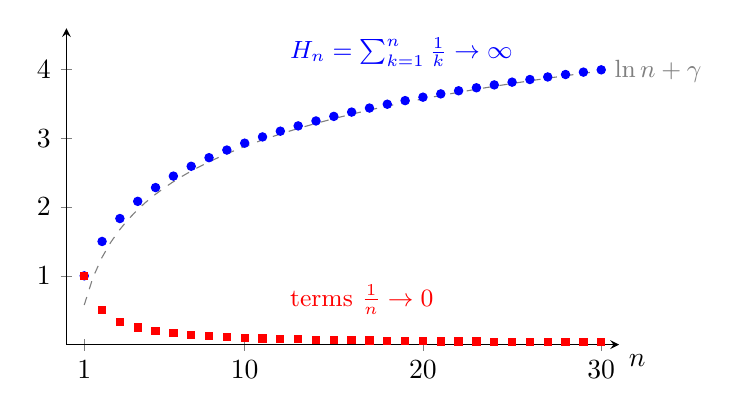
\begin{tikzpicture}
	\begin{axis}[
		axis lines=middle,
		xmin=0, xmax=31,
		ymin=0, ymax=4.6,
		xtick={1,10,20,30}, ytick={1,2,3,4},
		xlabel={$n$}, ylabel={},
		xlabel style={below right},
		clip=false,
		width=8.6cm, height=5.6cm
		]
		\addplot[gray, dashed, domain=1:30, samples=60] {ln(x)+0.5772};
		\node[gray, anchor=west, font=\small] at (axis cs:30.2,{ln(30)+0.5772}) {$\ln n+\gamma$};
		% H_n for n=1..30
		\addplot[only marks, mark=*, mark size=1.5pt, blue] coordinates {
			(1,1) (2,1.5) (3,1.8333) (4,2.0833) (5,2.2833) (6,2.45) (7,2.5929) (8,2.7179) (9,2.829) (10,2.929)
			(11,3.0199) (12,3.1032) (13,3.1801) (14,3.2516) (15,3.3182) (16,3.3807) (17,3.4396) (18,3.4951) (19,3.5477) (20,3.5977)
			(21,3.6454) (22,3.6908) (23,3.7343) (24,3.776) (25,3.816) (26,3.8544) (27,3.8915) (28,3.9272) (29,3.9617) (30,3.995)
		};
		\addplot[only marks, mark=square*, mark size=1.3pt, red, samples at={1,...,30}] {1/x};
		\node[blue, anchor=west, font=\small] at (axis cs:12,4.25) {$H_n=\sum_{k=1}^{n}\frac1k\to\infty$};
		\node[red, anchor=west, font=\small] at (axis cs:12,0.65) {terms $\frac1n\to 0$};
	\end{axis}
\end{tikzpicture}
\end{document}
